% !Mode:: "TeX:UTF-8"
% \textbf{计算专题------无取值说理、直接代入}

\begin{defproblem}{T16-A05-01}%
\begin{onlyproblem}%
先化简,再求值:$(x+2)(x-2)+(2x-1)^{2}-4x(x-1)$,其中$x=2\sqrt 3 $.
\end{onlyproblem}%
\begin{onlysolution}%
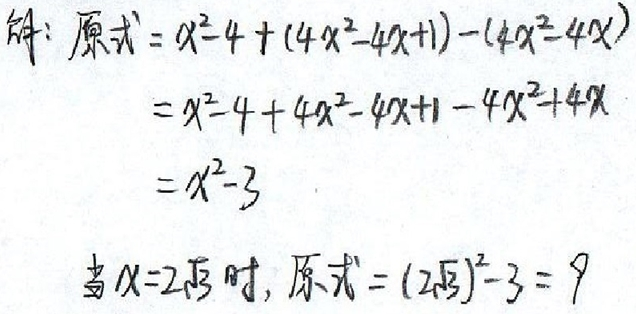
\includegraphics[width=8cm]{T16-A05-01-1.jpg}
\end{onlysolution}%
\end{defproblem}


\begin{defproblem}{T16-A05-02}%
\begin{onlyproblem}%
先化简,再求值:$(xy^2+x^2y)\cdot \dfrac{x}{x^2+2xy+y^2}\div \dfrac{x^2y}{x^2-y^2}$,其中$x=\pi ^0-\left(\dfrac{1}{2}\right)^{-1}$,$y=2\sin 45^{\circ}-\sqrt 8 $.

\end{onlyproblem}%
\begin{onlysolution}%

\end{onlysolution}%
\end{defproblem}


\begin{defproblem}{T16-A05-03}%
\begin{onlyproblem}%
先化简,再求值:$\left(x+2+\dfrac{3x+4}{x-2}\right)\div \dfrac{x^2+6x+9}{x-2}$,其中$x=2\sqrt 3 $.

\end{onlyproblem}%
\begin{onlysolution}%

\end{onlysolution}%
\end{defproblem}


\begin{defproblem}{T16-A05-04}%
\begin{onlyproblem}%
先化简,再求值:$\left(\dfrac{x^2-1}{x^2-2x+1}-x-1\right)\div \dfrac{x+1}{x-1}$,其中$x=2$.
\end{onlyproblem}%
\begin{onlysolution}%

\end{onlysolution}%
\end{defproblem}


\begin{defproblem}{T16-A05-05}%
\begin{onlyproblem}%
先化简,再求值:$3x^2y-\left[2xy^2-4\left(\dfrac{1}{2}xy-\dfrac{3}{4}x^2y\right)+xy\right]+3xy^2$,其中$x=3$,$y=-1$.
\end{onlyproblem}%
\begin{onlysolution}%

\end{onlysolution}%
\end{defproblem}


\begin{defproblem}{T16-A05-06}%
\begin{onlyproblem}%
先化简,再求值:$3x^{2}y[6xy-2(4xy-3)+3x^{2}y]+1$,其中$x$和$y$满足$\vert2x+1\vert+(y-2)^{2}=0$.
\end{onlyproblem}%
\begin{onlysolution}%

\end{onlysolution}%
\end{defproblem}

\begin{defproblem}{T16-A05-07}%
\begin{onlyproblem}%
(2019中考) 
先化简,再求值:$\left( {\dfrac{x+1}{x-2}-1} \right)\div \dfrac{x^2-2x}{x^2-4x+4}$,其中$x=\sqrt 3 $.
\end{onlyproblem}%
\begin{onlysolution}%
(2019中考)
\end{onlysolution}%
\end{defproblem}

